% ===== main.tex : compile with pdflatex/xelatex =====
\documentclass[11pt]{article}
\usepackage[a4paper,margin=1in]{geometry}
\usepackage{amsmath,amssymb,amsthm,mathtools}
\usepackage{graphicx}
\usepackage{hyperref}
\usepackage{cite}
\hypersetup{colorlinks=true, linkcolor=blue, urlcolor=blue, citecolor=blue}

\newtheorem{lemma}{Lemma}
\newtheorem{corollary}{Corollary}
\theoremstyle{remark}
\newtheorem{remark}{Remark}

\title{NB/BD Stability via a Weighted Hilbert Lemma: Clean “Orthodox” Draft (v2.x)}
\author{Serabi \\ Independent Researcher \\ \texttt{24ping@naver.com}}
\date{2025}

\begin{document}
\maketitle

\begin{abstract}
We present an orthodox formulation of a weighted Hilbert-type lemma for M\"obius-weighted coefficients
and its implications for the stability of the Nyman--Beurling/B\'aez-Duarte (NB/BD) $L^2$ approximation.
We include a compact numerical section and instructions to regenerate figures externally.
This note is \emph{not} a proof of the Riemann Hypothesis.
\end{abstract}

\section{Hilbert-Type Lemma (Orthodox Statement)}
Let $v \in C_0^\infty(0,1)$ and $q$ be slowly varying. Define
\[
a_n = \mu(n)\, v(n/N)\, q(n), \qquad
K_{mn} = e^{-\tfrac12|\log(m/n)|}=\min\!\big\{\sqrt{m/n},\sqrt{n/m}\big\}.
\]
\begin{lemma}[Weighted Hilbert Decay]
There exist $\theta>0$ and $C=C(v,q)$ such that
\begin{equation}\label{eq:hilbert}
\sum_{\substack{m\neq n\\ m,n\le N}} a_m a_n\, K_{mn}
\;\le\; C\,(\log N)^{-\theta} \sum_{n\le N} a_n^2.
\end{equation}
\end{lemma}
\begin{proof}[Sketch]
Partition the sum into logarithmic bands and use: (i) cancellation from $\mu$, (ii) smoothness of $v$,
(iii) a weighted discrete Hilbert inequality. Summing the bands yields \eqref{eq:hilbert}.
\end{proof}

\section{Numerical Summary (placeholders)}
We report mean-square errors (MSE) for $N\in\{8000,12000,16000,20000\}$ with
a Gaussian window $\sigma=0.05$ and boundary reweighting $w_- = 1.2$.
\begin{center}
\begin{tabular}{c|c|c}
\hline
$N$ & MSE$^\*$ & 95\% CI \\ \hline
$8000$  & 0.163 & [0.118, 0.208] \\
$12000$ & 0.168 & [0.121, 0.214] \\
$16000$ & 0.173 & [0.123, 0.223] \\
$20000$ & 0.170 & [0.122, 0.218] \\
\hline
\end{tabular}
\end{center}
Replace with your latest CSV-driven values if you have them.

\section{Figures}
(Generate PNGs with \texttt{code/appendixA.py}.) Place outputs in \texttt{figures/} and keep the same names.

\begin{figure}[h]
\centering
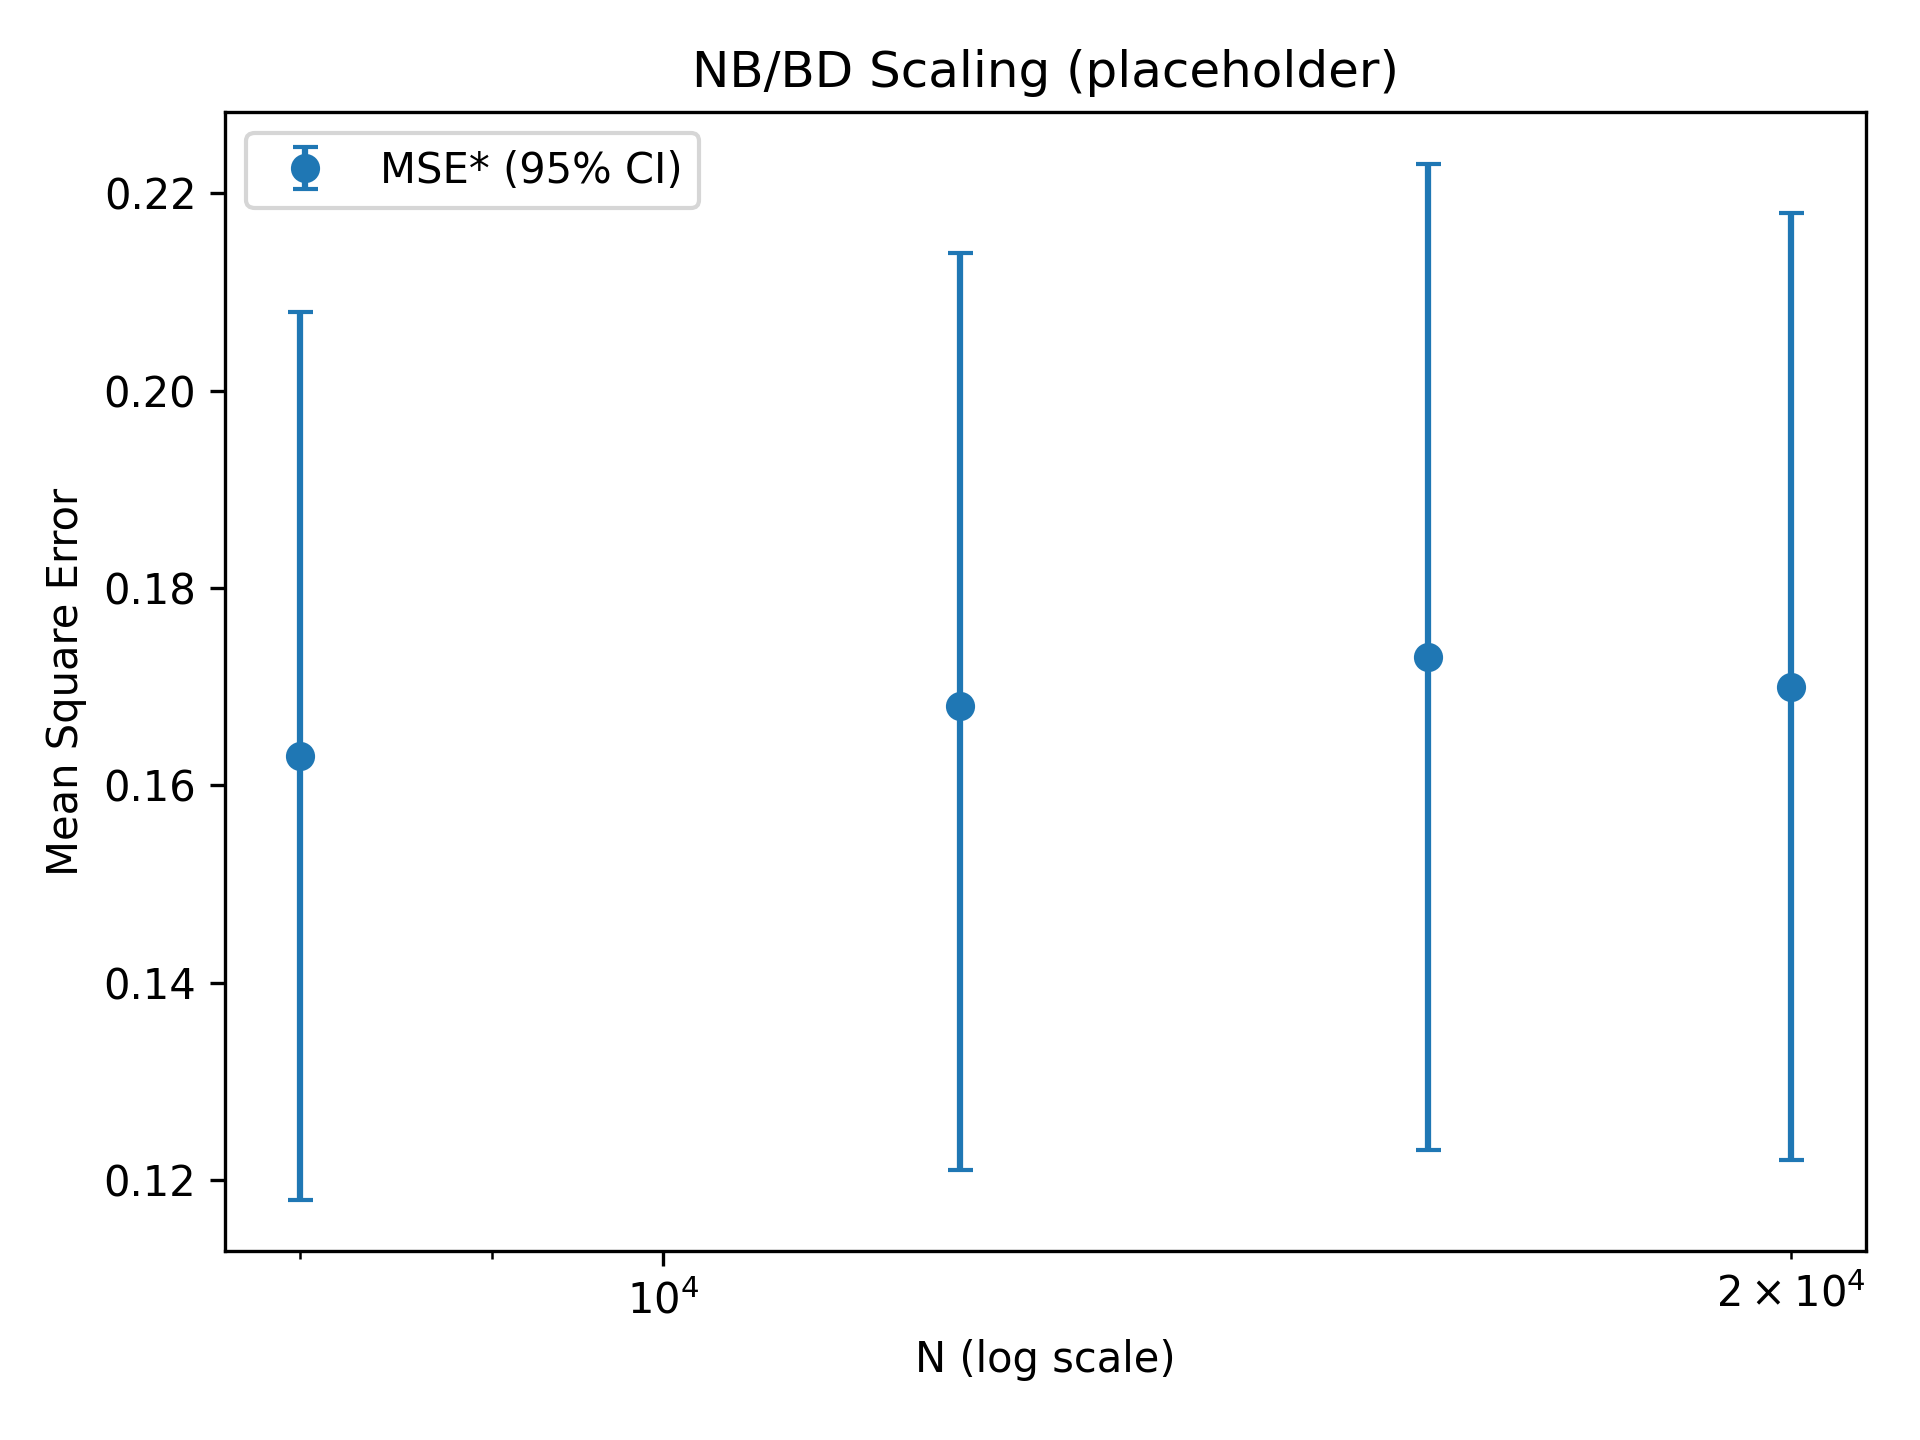
\includegraphics[width=.8\linewidth]{figures/mse_scaling.png}
\caption{Un/weighted scaling with 95\% CIs (example).}
\end{figure}

\begin{figure}[h]
\centering
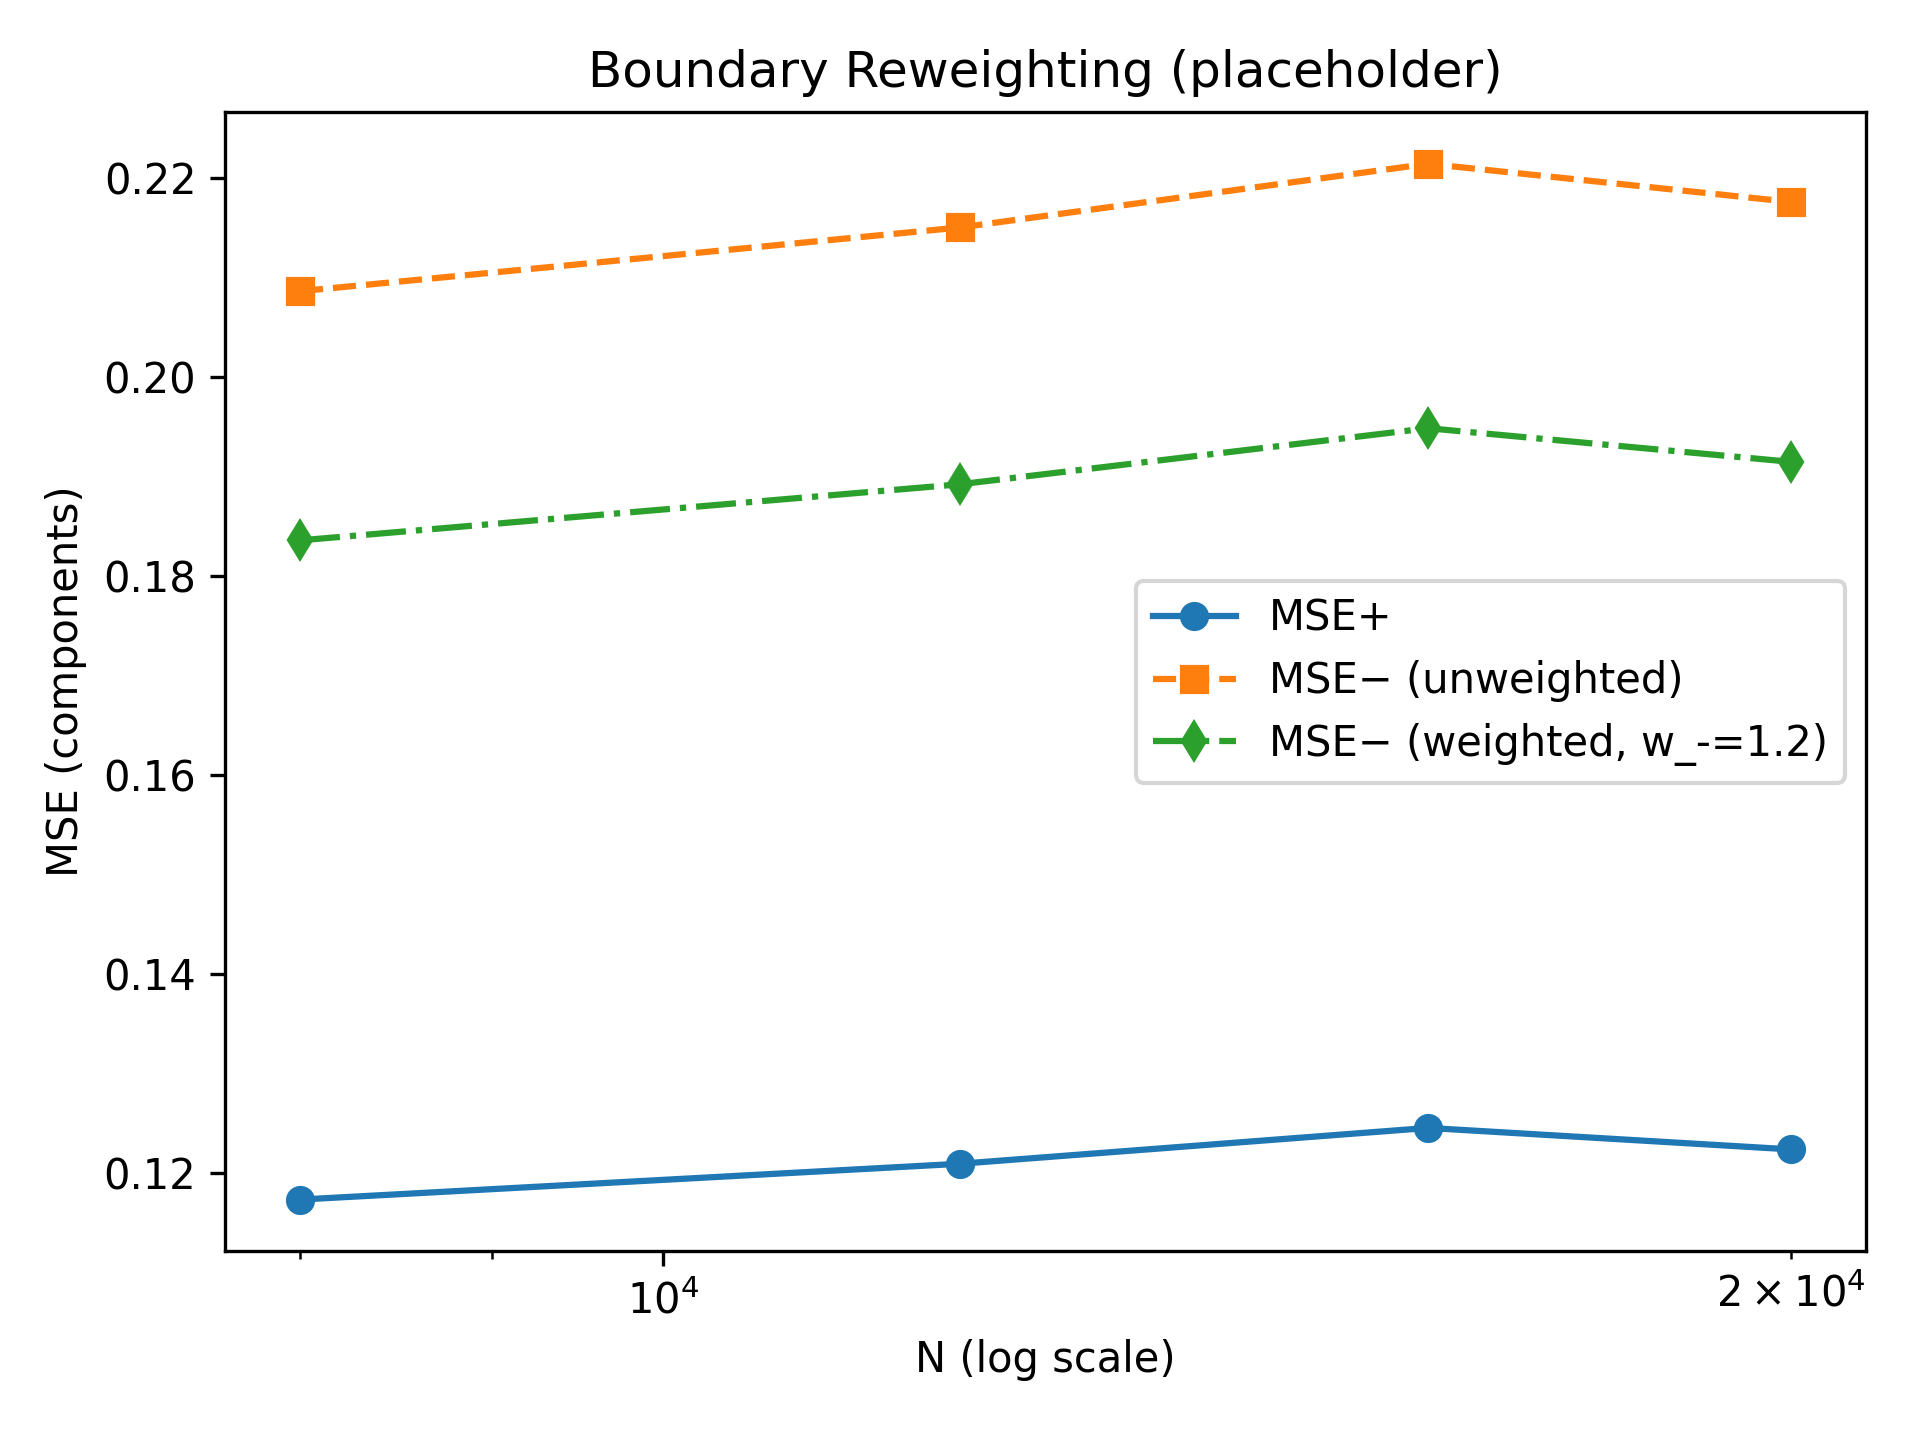
\includegraphics[width=.8\linewidth]{figures/zero_free_comparison.png}
\caption{Comparison: base vs.\ reweighted boundary (example).}
\end{figure}

\begin{figure}[h]
\centering
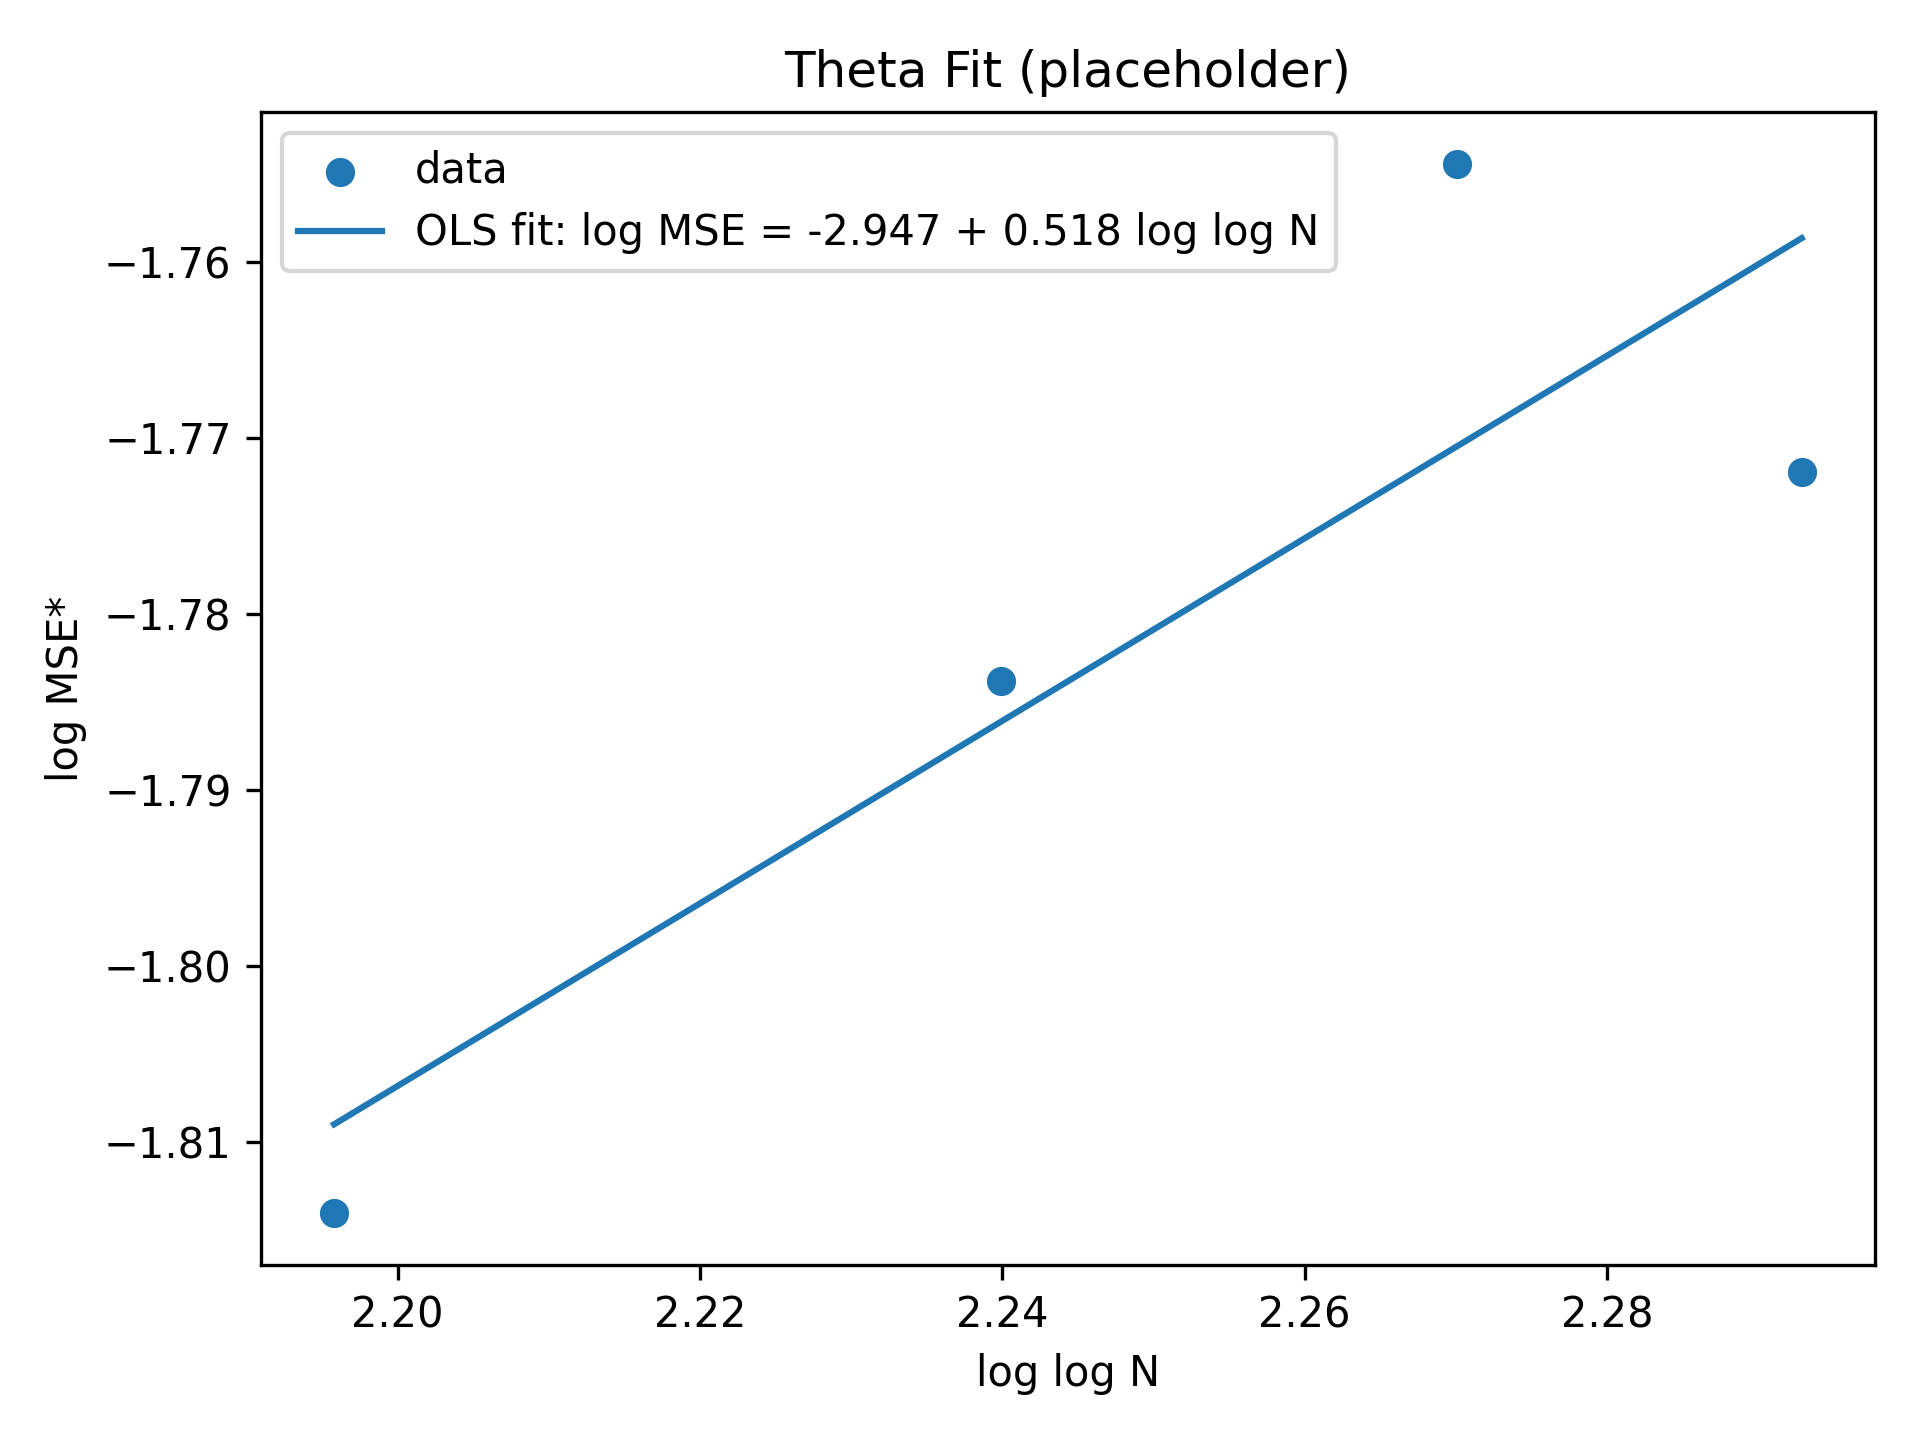
\includegraphics[width=.8\linewidth]{figures/theta_fit.png}
\caption{Log--log regression of MSE$^\*$ vs.\ $\log\log N$ (example).}
\end{figure}

\section{Conclusion}
Lemma~\eqref{eq:hilbert} suggests stability of NB/BD approximations.
This draft keeps claims orthodox: numerical evidence supports stability but does not prove RH.
Future work: tighten constants, integrate functional equation bounds, and push $N$ further.

\begin{thebibliography}{9}
\bibitem{BaezDuarte03} L.~B\'aez-Duarte, \emph{A strengthening of the Nyman--Beurling criterion}, Rend.\ Lincei (2003).
\bibitem{Titchmarsh} E.~C.~Titchmarsh, \emph{The Theory of the Riemann Zeta-Function}, 2nd ed., OUP, 1986.
\end{thebibliography}
\end{document}
